%%%%%%%%%%%%%%%%%%%%%%%%%%%%%%%%%%%%%%%%%%%%%%%%%%%%%%%%%%%%%%%%%%%%%
%%                                                                 %%
%% Please do not use \input{...} to include other tex files.       %%
%% Submit your LaTeX manuscript as one .tex document.              %%
%%                                                                 %%
%% All additional figures and files should be attached             %%
%% separately and not embedded in the \TeX\ document itself.       %%
%%                                                                 %%
%%%%%%%%%%%%%%%%%%%%%%%%%%%%%%%%%%%%%%%%%%%%%%%%%%%%%%%%%%%%%%%%%%%%%

%%\documentclass[referee,sn-basic]{sn-jnl}% referee option is meant for double line spacing

%%=======================================================%%
%% to print line numbers in the margin use lineno option %%
%%=======================================================%%

%%\documentclass[lineno,sn-basic]{sn-jnl}% Basic Springer Nature Reference Style/Chemistry Reference Style

%%======================================================%%
%% to compile with pdflatex/xelatex use pdflatex option %%
%%======================================================%%

%%\documentclass[pdflatex,sn-basic]{sn-jnl}% Basic Springer Nature Reference Style/Chemistry Reference Style

%%\documentclass[sn-basic]{sn-jnl}% Basic Springer Nature Reference Style/Chemistry Reference Style
\documentclass[pdflatex,sn-mathphys]{sn-jnl}% Math and Physical Sciences Reference Style
\usepackage{array}
\usepackage{caption}
\usepackage[font=small]{caption}
\captionsetup{justification=centering}

%%\documentclass[sn-aps]{sn-jnl}% American Physical Society (APS) Reference Style
%%\documentclass[sn-vancouver]{sn-jnl}% Vancouver Reference Style
%%\documentclass[sn-apa]{sn-jnl}% APA Reference Style
%%\documentclass[sn-chicago]{sn-jnl}% Chicago-based Humanities Reference Style
%%\documentclass[sn-standardnature]{sn-jnl}% Standard Nature Portfolio Reference Style
%%\documentclass[default]{sn-jnl}% Default
%%\documentclass[default,iicol]{sn-jnl}% Default with double column layout

%%%% Standard Packages
%%<additional latex packages if required can be included here>
%%%%

%%%%%=============================================================================%%%%
%%%%  Remarks: This template is provided to aid authors with the preparation
%%%%  of original research articles intended for submission to journals published 
%%%%  by Springer Nature. The guidance has been prepared in partnership with 
%%%%  production teams to conform to Springer Nature technical requirements. 
%%%%  Editorial and presentation requirements differ among journal portfolios and 
%%%%  research disciplines. You may find sections in this template are irrelevant 
%%%%  to your work and are empowered to omit any such section if allowed by the 
%%%%  journal you intend to submit to. The submission guidelines and policies 
%%%%  of the journal take precedence. A detailed User Manual is available in the 
%%%%  template package for technical guidance.
%%%%%=============================================================================%%%%

\jyear{2022}%

%% as per the requirement new theorem styles can be included as shown below
\theoremstyle{thmstyleone}%
\newtheorem{theorem}{Theorem}%  meant for continuous numbers
%%\newtheorem{theorem}{Theorem}[section]% meant for sectionwise numbers
%% optional argument [theorem] produces theorem numbering sequence instead of independent numbers for Proposition
\newtheorem{proposition}[theorem]{Proposition}% 
%%\newtheorem{proposition}{Proposition}% to get separate numbers for theorem and proposition etc.

\theoremstyle{thmstyletwo}%
\newtheorem{example}{Example}%
\newtheorem{remark}{Remark}%

\theoremstyle{thmstylethree}%
\newtheorem{definition}{Definition}%

\raggedbottom
%%\unnumbered% uncomment this for unnumbered level heads

\begin{document}

\title[Red Blood Cell Lab]{Measurement of Key Metrics on Red Blood Cells in a Blood Sample.}

\author*[1,2]{\fnm{Harsh} \sur{Agrawal}}\email{ha1822@ic.ac.uk}

\affil*[1]{\orgdiv{Molecular Bioengineering}, \orgname{Imperial College London}}

\abstract{The purpose of this set of experiments was to determine the concentration of RBCs/volume in a given blood sample, measure the hematocrit, calculation of Mean Cell Volume (MCV), Mean Cellular Haemoglobin (MCH), and Mean Cellular Haemoglobin Concentration (MCHC).}



\maketitle

\section{Experiment 1}\label{sec1}
\subsection{Obtaining the RBC Count}
For the RBC count, 5$\mu$L of blood sample was extracted and diluted in 995$\mu$L of Hayem's solution (carrying out a 1:200 dilution). A small volume of this diluted sample was transferred to the hemocytometer slide and then the cells were counted under a microscope.\vspace{2mm}

$\Rightarrow$ Total RBCs counted over 5 medium-sized squares:

\[Count: 527. mean(\mu): 105.4, std. \, dev.(\sigma): 5.122). \]\vspace{0.3mm}

$\Rightarrow$ Total Volume of the 5 medium-sized squares:
\[5 * 0.004mm^{3} = 2 * 10^{-8} Litres\]

$\Rightarrow$ Accounting for the dilution, the total RBC count per Litre:

\[\frac{527 * 200}{2 * 10^{-8}} = 5.27 * 10^{12} RBC/L\]\vspace{0.3mm}

Since the blood was drawn from a male volunteer in our group, the count is under the normal range of RBC count.

\subsection{Obtaining the Haematocrit and Haemoglobin Concentration}

A small percentage of blood was transferred to a capillary tube, centrifuged, and read under a micro-hematocrit reader to obtain the following measurement:

\[Haematocrit = 44\%\]\vspace{0.3mm}

A small blood sample was collected with the help of a HaemoCue cuvette and the recording was obtained from the reader.

\[[Hb] =  144g/L\]\vspace{0.3mm}

\textit{*Due to time constraints, we weren't able to obtain multiple measurements.}

\subsection{Calculation of Derived Red Blood Cell Parameters}
$\Rightarrow$ Mean Cell Volume (MCV):

\[MCV = \frac{Hct}{RBC * 100}L =  \frac{0.44}{5.27 * 10^{12}} = 83.5 fL\]\vspace{2mm}

\noindent $\Rightarrow$ Mean Cellular Haemoglobin (MCH):
\[MCH = \frac{Hb}{RBC}g = \frac{144}{5.27 * 10^{12}}g = 27.32 pg\]\vspace{2mm}

\noindent $\Rightarrow$ Mean Cellular Haemoglobin Concentration (MCHC):

\[MCHC = \frac{Hb * 100}{Hct}g/L = \frac{144 * 100}{44} = 327.27g/L\]
All the calculated RBC parameters (MCV, MCH, and MCHC) are under the normal range of a healthy male adult.
\newpage

\section{Questions }
\subsection{Comparison of RBC Parameters in Male and Female Students}
\textbf{Hypothesis 1: Males Students have a higher haemoglobin concentration than female students}
\begin{figure}[hp]
    \centering
    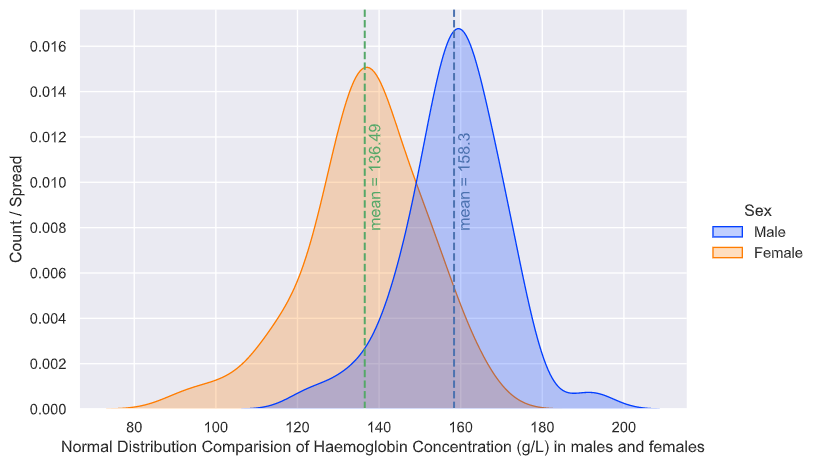
\includegraphics[width=0.8\textwidth]{photos/hyp_1.png}
    \caption{Comparison of Haemoglobin Concentration (g/L) in male vs. female students. The graph was plotted using the seaborn library in python. }\label{fig1}
\end{figure}
\vspace{-15pt}

It can clearly be observed that the mean haemoglobin concentration of male students (158.3g/L) is visibly higher than female students(136.49g/L). \textbf{\textit{Thus we can't reject the given hypothesis.}}
\\

\noindent\textbf{Hypothesis 2: Males Students have a higher Mean Cell Volume than female students}
\begin{figure}[h!]
    \centering
    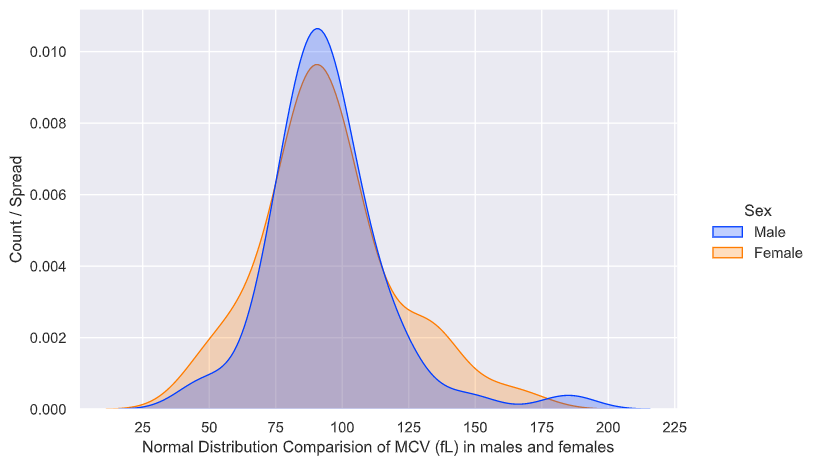
\includegraphics[width=0.8\textwidth]{photos/hyp_2.png}
    \caption{Comparison of Mean Cell Volume (fL) in male vs. female students. }\label{fig1}
\end{figure}

Unlike hypothesis 1, we can clearly observe an overlap of the mean cell volume of male students (94.2g/L) and female students(94.3g/L).

\textbf{\textit{Thus we can reject the given hypothesis.}}
\subsection{Components and Functions of Blood}
Blood is one of the most critical components of our body. It is responsible for carrying out various vital functions such as the transport of oxygen, nutrients, generated waste, etc. It is comprised of four major segments:
\begin{itemize}
    \item Plasma: Plasma is the liquid component of blood and is ~55\% of the total volume. It houses various essential metabolites and proteins and is required for the maintenance of pH, regulation of osmotic pressure, etc.
    \item Erythrocytes: Also referred to as Red Blood Cells, comprise 40-45\% of the blood volume. They are responsible to give blood its dark red color. These cells contain hemoglobin that is required to carry Oxygen from the lungs to the rest of the body.
    \item  Leukocytes: Also referred to as White Blood Cells, they are one of the primary components of our immune system. These comprise of 1\% of the total volume.
    \item Thrombocytes: Also referred to as thrombocytes, these make up <1\% of the total blood volume and are responsible for blood clotting.
\end{itemize}

\subsection{Estimation of Oxygen concentration in 1L of blood.}
Average RBC count (mean $\pm$ std. dev) of a healthy human (male and female combined): \(4.5 * 10^{12} {\pm} 0.5 * 10^{12} RBC/L\)\footnote{A combined mean $\pm$ standard deviation was calculated using the average values taken for males and females individually from \href{https://www.nhs.uk/conditions/red-blood-count/}{https://www.nhs.uk/conditions/red-blood-count/}}.

Total O\textsubscript{2} concentration:

\[\Rightarrow\frac{RBCs}{litre} * \frac{haemoglobin}{cell} * \frac{O\textsubscript{2}}{haemoglobin}\]

\[\Rightarrow(4.5\pm 0.6) * 10^{12} * 3 * 10^{8} * 4 = (5.4\pm 0.6) * 10^{21}\,molecules/L\]
The concentration of O\textsubscript{2} according to the calculated value above:

\[\frac{(5.4\pm 0.6)*10^{21}}{6.023 * 10^{23}} = (8.96\pm0.99) * 10^{-3} M = 8950\pm990 {\mu}M\]\vspace{1mm}


Compared to 225$\mu$M of O\textsubscript{2} of dissolved air-saturated saline (DASS) solution, the concentration of O\textsubscript{2} in the blood is significantly high. This point to the greater blood-carrying capacity of blood due to the presence of haemoglobin molecules.


\subsection{Principle of Oxygen Saturation Measurement}
Hemoglobin is composed of 4 subunits (2 alpha, 2 beta in adults) and exists in two forms\footnote{Taken from: \href{https://medicine.uiowa.edu/iowaprotocols/pulse-oximetry-basic-principles-and-interpretation}{https://medicine.uiowa.edu/iowaprotocols/pulse-oximetry-basic-principles-and-interpretation}.}:
\begin{itemize}
    \item Taut (T): \textit{de-oxygenated form} with low affinity for O2, therefore it promotes the release/unloading of O2.
    \item Relaxed (R): \textit{ oxygenated form} with high affinity for O2, therefore oxygen loading is favored.
\end{itemize}
T and R configurations lead to different electromagnetic absorption and therefore different emission of light. Oxymeters exploit this advantage to determine the oxygen saturation in the blood.
Two bands of LED - A red led, with a wavelength of 660 nm, and the other infrared, with a wavelength of 940 nm - strike light through the skin and observe the absorbance of both the light waves. Oxygenated hemoglobin absorbs more infrared light and \textit{allows more red light} to pass through whereas deoxygenated hemoglobin\textit{ allows more infrared light }to pass through and absorbs more red light.
Multiple readings are recorded and then the ratio is calculated between red and infrared light to obtain SpO\textsubscript{2} from Beer-Lambert Law\footnote{Taken from \href{https://www.frca.co.uk/article.aspx?articleid=332}{https://www.frca.co.uk/article.aspx?articleid=332}}.

Some watches also have an additional green light that is absorbed by other components of the blood. It is used to correct observation for skin color, thickness, and other factors that may differ from person to person. It improves the accuracy of the red and infrared readings.
\end{document}
